\chapter{Arhitektura sustava}

Blok dijagram arhitekture PDH sustava dan je na slici \ref{fig:fersat_blok}.

\begin{figure}[H]
	\centering
	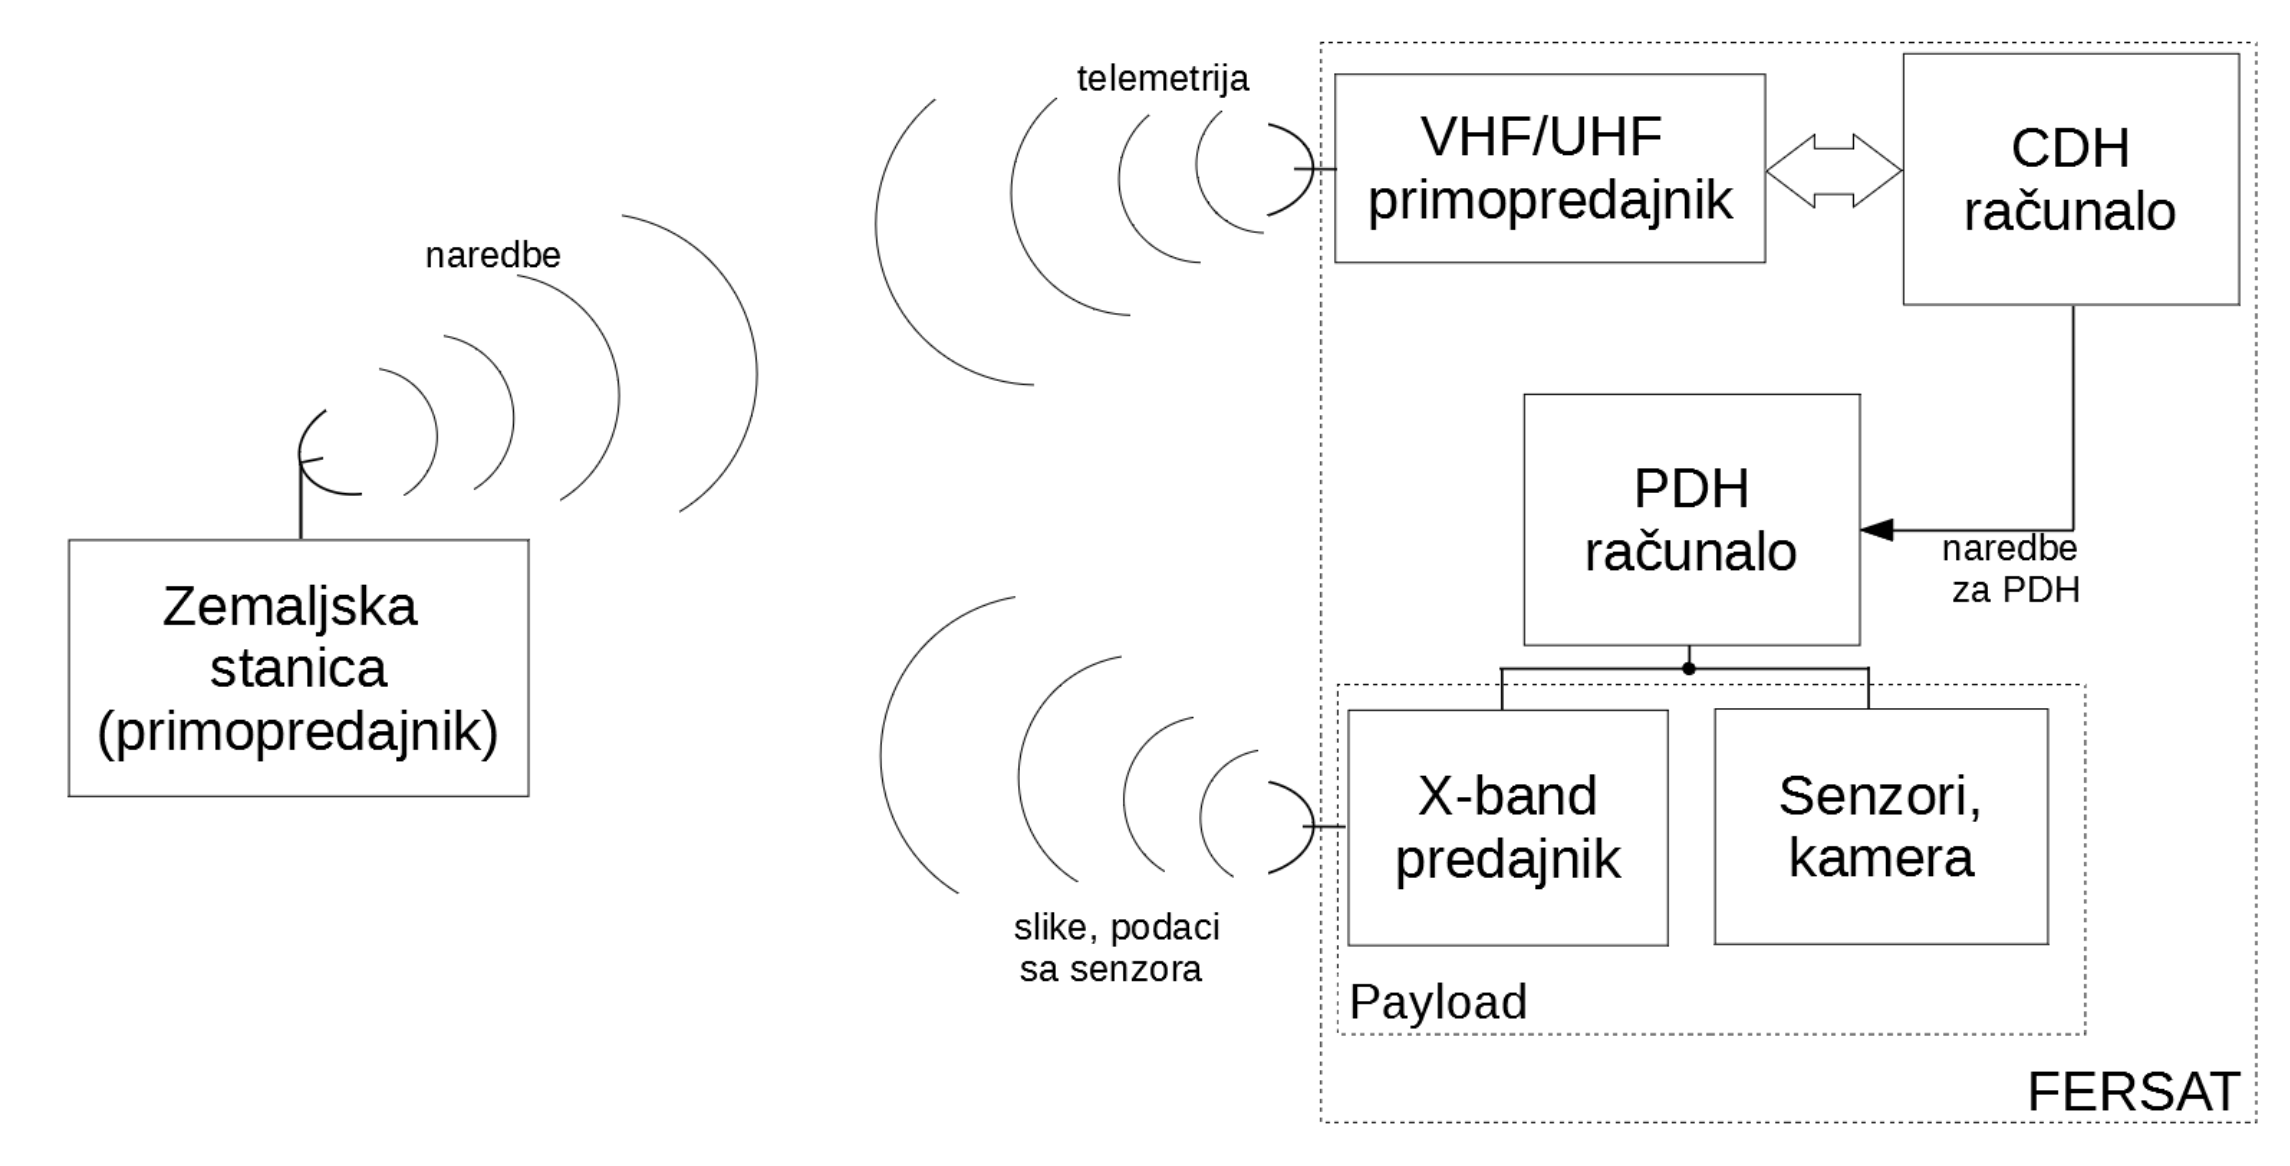
\includegraphics[width=\textwidth]{fersat_blok_dijagram.png}
	\caption{Blok dijagram arhitekture PDH sustava}
	\label{fig:fersat_blok}
\end{figure}

Slanjem određenog signala na sklop za kameru može se uslikati fotografija, a nakon fotografiranja fotografija se pohranjuje na vlastiti međuspremnik kamere. Cilj je spremljenu fotografiju pročitati iz međuspremnika kamere i spremiti ju na \textit{flash} memoriju koja se nalazi na pločici PDH-a, gdje može biti spremljena dok se ne zatraži slanje slike preko X-band predajnika na Zemlju.

\textit{Flash} memorija, osim što služi za pohranu slike, služi i za pohranu podataka s drugih senzora. Ona prima i šalje podatke ovisno o poslanoj naredbi putem SPI komunikacije s mikrokontrolerom.

Upravljačko sklopovlje PDH računala se sastoji od STM32F471VGT6 mikrokontrolera, spomenute vanjske \textit{flash} memorije, konektora za povezivanje s ostalim dijelovima sustava (uključujući i konektor za povezivanje s kamerom), sustava za napajanje, upravljačkog sklopovlja za CAN komunikaciju i sklopa za kontrolu izvođenja programa (engl. \textit{watchdog}) \cite{zavrsni_filip_juric}. Izgled tiskane pločice upravljačkog sklopovlja PDH računala prikazan je na slikama \ref{fig:PDH_PCB_1} i \ref{fig:PDH_PCB_2}. Konektor X1 služi za povezivanje sustava s kamerom.

\begin{figure}[H]
	\centering
	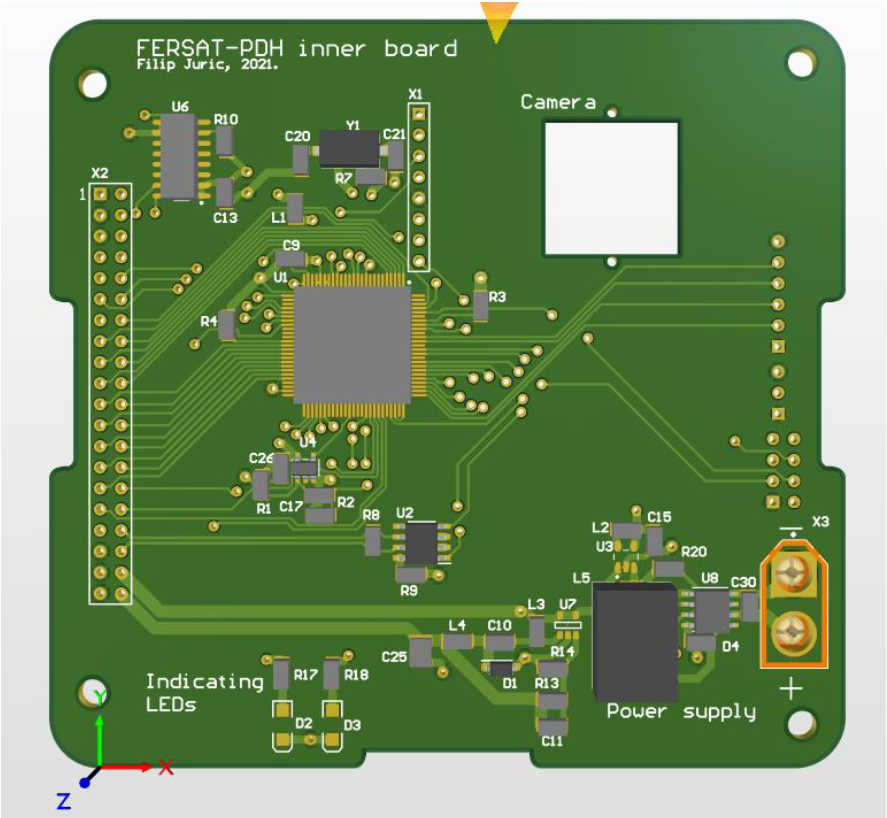
\includegraphics[height= 9 cm]{PDH_PCB_1.PNG}
	\caption{Prikaz gornje strane tiskane pločice upravljačkog sklopovlja PDH računala \cite{zavrsni_filip_juric}}
	\label{fig:PDH_PCB_1}
\end{figure}

\begin{figure}[H]
	\centering
	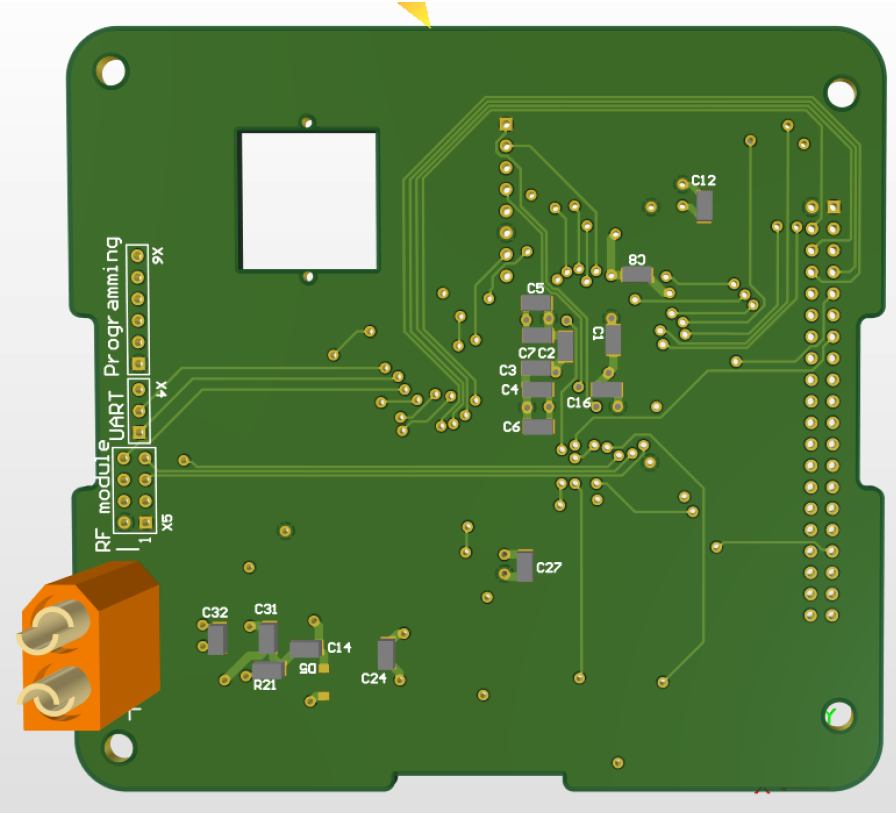
\includegraphics[height= 9 cm]{PDH_PCB_2.PNG}
	\caption{Prikaz donje strane tiskane pločice upravljačkog sklopovlja PDH računala \cite{zavrsni_filip_juric}}
	\label{fig:PDH_PCB_2}
\end{figure}

Programska podrška za PDH računalo već je razvijena \cite{diplomski_goran_petrak}. Međutim, u međuvremenu je došlo do promjene izbora mikrokontrolera PDH računala, te je stoga postojeću programsku podršku bilo potrebno prilagoditi trenutačnom sklopovlju.